\scanpage{112}
% ms. line 01
Notons que si $-\theta\leq\arg z\leq+\theta$, où $\theta$ est
% ms. line 02
un angle arbitraire que nous prendrons une
% ms. line 03
fois pour toutes entre $\frac{\pi}{3}$ et $\pi$, on
% ms. line 04
aura $x\geq c|z|$, où $c$ est une
% ms. line 05
constante $>0$, d'où \deleted{$f(z)\geq$}
\figure{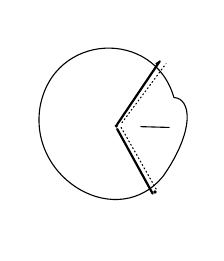
\begin{tikzpicture}[x=1cm,y=1cm,line cap=round]
\draw (0,0) .. controls (-.25,.88) and (-1.53,.83) .. (-1.70,-.12) .. controls (-1.85,-1.05) and (-.7,-1.71) .. (-.13,-.99) .. controls (.27,-.41) and (.22,-.01) .. (0,0);
\draw[thick] (-.72,-.34)--(-.18,.46);
\draw[thick] (-.72,-.40)--(-.27,-1.22);
\draw[densely dotted] (-.66,-.32)--(-.10,.43) (-.67,-.38)--(-.21,-1.19);
\draw[thin] (-.42,-.37)--(-.06,-.38);
\fill (-.73,-.36) circle (.024) (-.21,.43) circle (.025) (-.24,-1.20) circle (.025);
\end{tikzpicture}}
% ms. line 06
\[ |f(z)|\geq e^{c|z|}|z|^m\prod_i\left|1-\frac z{z_i}\right|\qquad\text{qnd }-\theta\leq\arg z\leq+\theta \]

% ms. line 07
D'autre part on a $|f(z)|\leq|h(z)|\leq \mathrm c^{\mathrm{te}}\times e^{\varepsilon|z|}$
% ms. line 08
d'où, en supposant qu'on ait choisi $\varepsilon<c$
% ms. line 09
\[ |z|^m\prod_i\left|1-\frac{z}{z_i}\right|\leq k e^{-\alpha|z|} \]
% ms. line 10
où $\alpha>0$, dès que $-\theta\leq\arg z\leq+\theta$.

% ms. line 11
Posons $g(z)=z^m\prod_i(1-\frac z{z_i})$, notre formule
% ms. line 12
s'écrit \quad \uline{$|g(z)|\leq ke^{-\alpha|z|}$} \quad si $-\theta\leq\arg z\leq+\theta$

% ms. line 13
Montrons qu'une \deleted{telle} inégalité n'est possible
% ms. line 14
pour une fonction $g$ de genre zéro que si elle
% ms. line 15
est \deleted{\unsure{identique}} \inserted{constante}. On a en effet aussi, $g$ étant de genre
% ms. line 16
zéro \qquad $|g(z)|\leq k'e^{\frac{\alpha}{3}|z|}$ \qquad pour l'ensemble
% ms. line 17
Posons $\omega=e^{2i\pi/3}$, et $G(z)=g(z)g(\omega z)g(\omega^{\unsure{2|3}}z)$
% ms. line 18
C'est une fonction entière, et on vérifie
% ms. line 19
aussitôt que, \uline{quel que soit $z$}, on a
% ms. line 20
\[ |G(z)|\leq(ke^{-\alpha|z|})(k'e^{\frac{\alpha}{3}|z|})(k'e^{\frac{\alpha}{3}|z|})=k''e^{-\frac{\alpha}{3}|z|} \]
% ms. line 21
$G(z)$ serait donc bornée, donc une constante.
% ms. line 22
Mais $G(z)=z^{\unsure{3m}}\prod_i\left(1-\frac{z^3}{z_i^3}\right)$, il
% margin note written sideways
% ms. line 23
\margin{\unsure{faudra|faut donc} que l'ens. d'indices $i$ soit vide, et $m=0$, donc que $g(z)$ soit une constante. \unsure{Cela|Cel.|Ceci} signifie que $f(z)=\mathrm C^{\mathrm{te}}e^{\beta z}$, ce qui est incompatible avec $|f(z)|\leq|\deleted{\unsure{g}}h(z)|\leq \mathrm c^{\mathrm{te}}e^{\varepsilon|z|}$.}
% archive sheet number: 113
